\section{TIG Design}
\justify{The TIG Stack is built over K8s\footnote{https://github.com/lsst-it/gi-k8s}, but for servers, a telegraf service agent needs to be setup in each one. To accomplish this, the server's configuration was performed through puppet, which is a software configuration management tool that includes its own declarative language to describe the system configuration.}
\vskip 2cm
\begin{figure}
  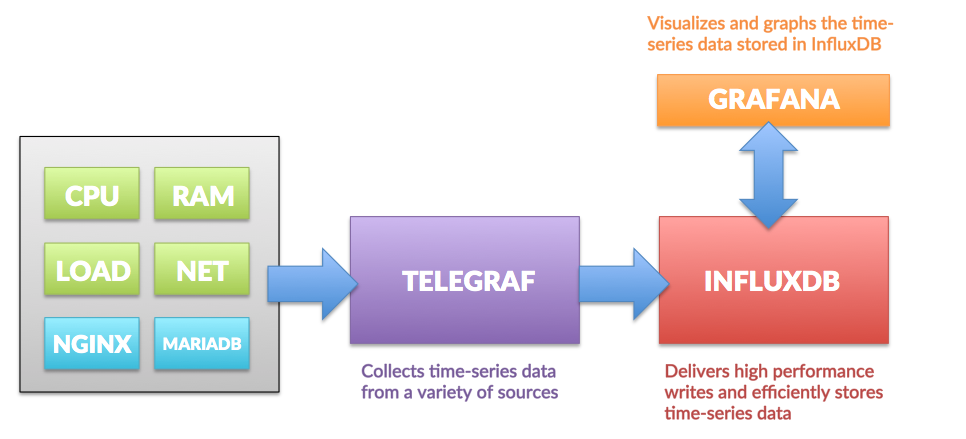
\includegraphics[width=14cm]{images/image1.png}
  \centering
  \caption{Telegraf, InfluxDB, and Grafana operational diagram}
\end{figure}
\vskip 2cm
\justify{As the diagram shows\footnote{https://www.jorgedelacruz.es/2020/11/23/en-busca-del-dashboard-perfecto-influxdb-telegraf-y-grafana-parte-i-instalando-influxdb-telegraf-y-grafana-sobre-ubuntu-20-04-lts/}, Telegraf picks up the metrics - such as CPU, RAM, Network Traffic, Load - and send them over InfluxDB. InfluxDB stores the metrics into a DB, to then be read by Grafana, which is capable of display real-time dashboards and plots.}

\newpage
\subsection{Telegraf Puppet's configuration}
\justify{On every server, the following puppet profile configuration is passed:}
\begin{lstlisting}
class { 'telegraf':
  hostname => $facts['networking']['fqdn'],
  outputs  => {
    'influxdb' => [{
        'urls'     => [$url],
        'database' => $database,
        'username' => $username,
        'password' => $password,
    }]
  },
  inputs   => {
    'cpu'    => [{
        'percpu'   => true,
        'totalcpu' => true,
    }],
    'mem'    => [{}],
    'io'     => [{}],
    'net'    => [{}],
    'disk'   => [{}],
    'swap'   => [{}],
    'system' => [{}],
  }
}
\end{lstlisting}
\justify{This will signal the server to install the latest telegraf package, setup the configuration file with the provided fields and ensure that the Telegraf's Service is running. All the metrics are then send to InfluxDB to be process and store.}

\newpage
\subsection{Telegraf over K8s}
\justify{On the other hand, network devices are not capable - at the time - of running telegraf as a service, so to be able to fetch the network device's metrics, a Telegraf intance is needed. In terms of reliability, it's better to have it over k8s than a VM. For this deployment, the following yaml charts were used:}
\begin{itemize}
  \item \textbf{ConfigMap:} Passes the content for the \textit{telegraf.conf} file to the Pod.
  \item \textbf{Deployment:} Generates a Pod with a container that withholds the telegraf docker image.
  \item \textbf{Role:} A Role to handle telegraf.
  \item \textbf{Service Account:} A Service Account to handle telegraf
  \item \textbf{Role Binding:} Enrolls and puts together the telegraf Service Account and Role
  \item \textbf{Service:} Creates and manage the telegraf service, as it would a Linux OS.
\end{itemize}
\subsection{InfluxDB over K8s}

\subsection{Grafana over K8s}

\newpage